\chapter{Results and Discussion}

\section{Time calibration}

In this part a suitable calibration to transform the channel axis to a time axis is determined. In order to collect appropriate measurements for that, the moveable detector is fixed at the minimal distance from the source, an the discriminator threshold is set to a value of 55, so that most $\SI{511}{keV}$ quanta are detected, but any noise is cut off. The manual delay of the TPC is set to $\Delta t = \SI{2}{ns}$ which works as the zero value. Now, the spectrum is measured at multiple manual delay times, from $\Delta t = \SIrange[]{0}{32}{ns}$ with a distance of \SI{4}{ns} each. A measured spectrum can be seen in figure \ref{fig:0nsnofit}.

\begin{figure}[H]
    \centering
    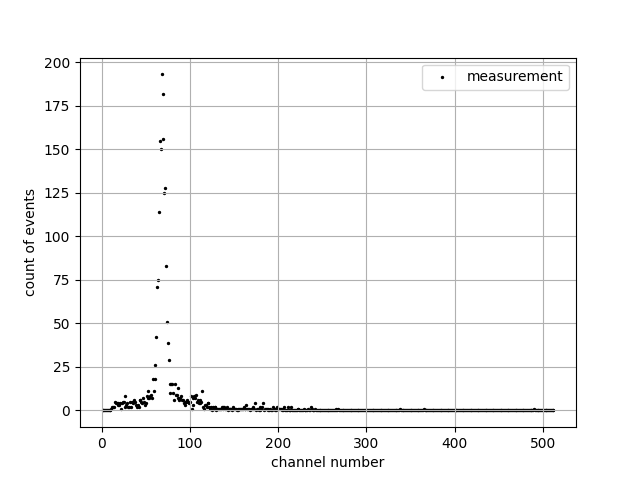
\includegraphics[width=110mm,scale=0.5]{Positronium/include/0nsnofit.png}
    \caption{Measured time sprectum at 0ns manual delay} 
    \label{fig:0nsnofit}
\end{figure}

For each of the time spectra, the peak is fitted to a gaussian distribution to find out its channel number. For each fit an uncertainty of 3 is assumed on the channel, the figures of this can be found in the appendix. The set of peak channel numbers can then be linearly fitted to the manual delay time with this function: 
$$ t = a\cdot\mu +b$$
where $\mu$ is the peak channel number and $a,b$ parameters to be determined.